\documentclass[PLAIN]{Lilly}
\begin{document}
\pagenumbering{arabic}
\tableofcontents \clearpage 
\begin{lstplain}[language=lLatex]
%%Einbindung erfolgt über:
\getGraphics{:lan:Pfad:ran:}
 \end{lstplain}
\begin{tabularx}{\linewidth}{^m{0.5\linewidth}^>{\centering\arraybackslash}X+}
\toprule\headerrow Pfad & Ergebnis\\
\midrule

\phantomsection \addcontentsline{toc}{chapter}{Allerlei}
\phantomsection \addcontentsline{toc}{section}{Teufel}\verb|Allerlei/Teufel| & \getGraphics{Allerlei/Teufel}\\
\midrule 
\phantomsection \addcontentsline{toc}{chapter}{Automat}
\phantomsection \addcontentsline{toc}{section}{AutomatDFA}\verb|Automat/AutomatDFA| & \getGraphics{Automat/AutomatDFA}\\
\midrule \phantomsection \addcontentsline{toc}{section}{AutomatNFA}\verb|Automat/AutomatNFA| & \getGraphics{Automat/AutomatNFA}\\
\midrule \phantomsection \addcontentsline{toc}{section}{CYK-Beispiel/CYKBeispiel1}\verb|Automat/CYK-Beispiel/CYKBeispiel1| & \getGraphics{Automat/CYK-Beispiel/CYKBeispiel1}\\
\midrule \phantomsection \addcontentsline{toc}{section}{CYK-Beispiel/CYKBeispiel2}\verb|Automat/CYK-Beispiel/CYKBeispiel2| & \getGraphics{Automat/CYK-Beispiel/CYKBeispiel2}\\
\midrule \phantomsection \addcontentsline{toc}{section}{CYK-Beispiel/CYKBeispiel3}\verb|Automat/CYK-Beispiel/CYKBeispiel3| & \getGraphics{Automat/CYK-Beispiel/CYKBeispiel3}\\
\midrule \phantomsection \addcontentsline{toc}{section}{CYK-Beispiel/CYKBeispiel4}\verb|Automat/CYK-Beispiel/CYKBeispiel4| & \getGraphics{Automat/CYK-Beispiel/CYKBeispiel4}\\
\midrule \phantomsection \addcontentsline{toc}{section}{CYK-Beispiel/CYKBeispiel5}\verb|Automat/CYK-Beispiel/CYKBeispiel5| & \getGraphics{Automat/CYK-Beispiel/CYKBeispiel5}\\
\midrule \phantomsection \addcontentsline{toc}{section}{CYK-Beispiel/CYKBeispiel6}\verb|Automat/CYK-Beispiel/CYKBeispiel6| & \getGraphics{Automat/CYK-Beispiel/CYKBeispiel6}\\
\midrule \phantomsection \addcontentsline{toc}{section}{CYKAlgorithmus}\verb|Automat/CYKAlgorithmus| & \getGraphics{Automat/CYKAlgorithmus}\\
\midrule \phantomsection \addcontentsline{toc}{section}{Demo-1}\verb|Automat/Demo-1| & \getGraphics{Automat/Demo-1}\\
\midrule \phantomsection \addcontentsline{toc}{section}{Demo-2}\verb|Automat/Demo-2| & \getGraphics{Automat/Demo-2}\\
\midrule \phantomsection \addcontentsline{toc}{section}{Demo}\verb|Automat/Demo| & \getGraphics{Automat/Demo}\\
\midrule \phantomsection \addcontentsline{toc}{section}{Header}\verb|Automat/Header| & \getGraphics{Automat/Header}\\
\midrule \phantomsection \addcontentsline{toc}{section}{MealyAutomat}\verb|Automat/MealyAutomat| & \getGraphics{Automat/MealyAutomat}\\
\midrule \phantomsection \addcontentsline{toc}{section}{MooreAutomat}\verb|Automat/MooreAutomat| & \getGraphics{Automat/MooreAutomat}\\
\midrule 
\phantomsection \addcontentsline{toc}{chapter}{Datenbanken}
\phantomsection \addcontentsline{toc}{section}{ERMExample}\verb|Datenbanken/ERMExample| & \getGraphics{Datenbanken/ERMExample}\\
\midrule 
\phantomsection \addcontentsline{toc}{chapter}{Eigene}
\phantomsection \addcontentsline{toc}{section}{Proseminar/Cluster/en-circles}\verb|Eigene/Proseminar/Cluster/en-circles|\quad{\tiny pdf}& 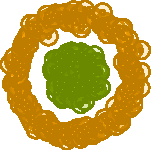
\includegraphics[width=0.8\linewidth]{Eigene/Proseminar/Cluster/en-circles.pdf}\\
\midrule \phantomsection \addcontentsline{toc}{section}{Proseminar/Cluster/en-clusters}\verb|Eigene/Proseminar/Cluster/en-clusters|\quad{\tiny pdf}& 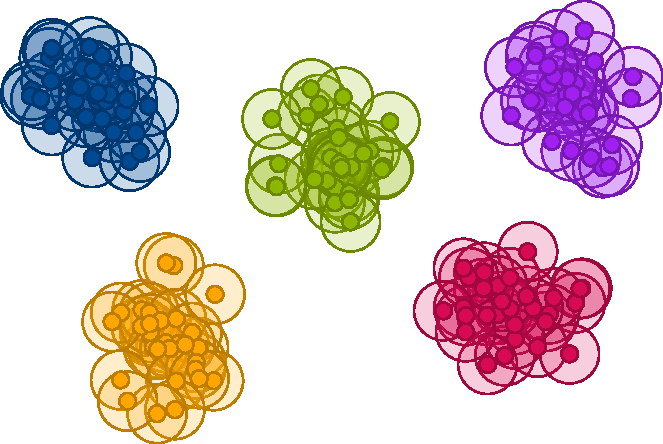
\includegraphics[width=0.8\linewidth]{Eigene/Proseminar/Cluster/en-clusters.pdf}\\
\midrule \phantomsection \addcontentsline{toc}{section}{Proseminar/Cluster/en-moons}\verb|Eigene/Proseminar/Cluster/en-moons|\quad{\tiny pdf}& 
\includegraphics[width=0.8\linewidth]{Eigene/Proseminar/Cluster/en-moons.pdf}\\
\midrule \phantomsection \addcontentsline{toc}{section}{Proseminar/Cluster/en-special}\verb|Eigene/Proseminar/Cluster/en-special|\quad{\tiny pdf}& 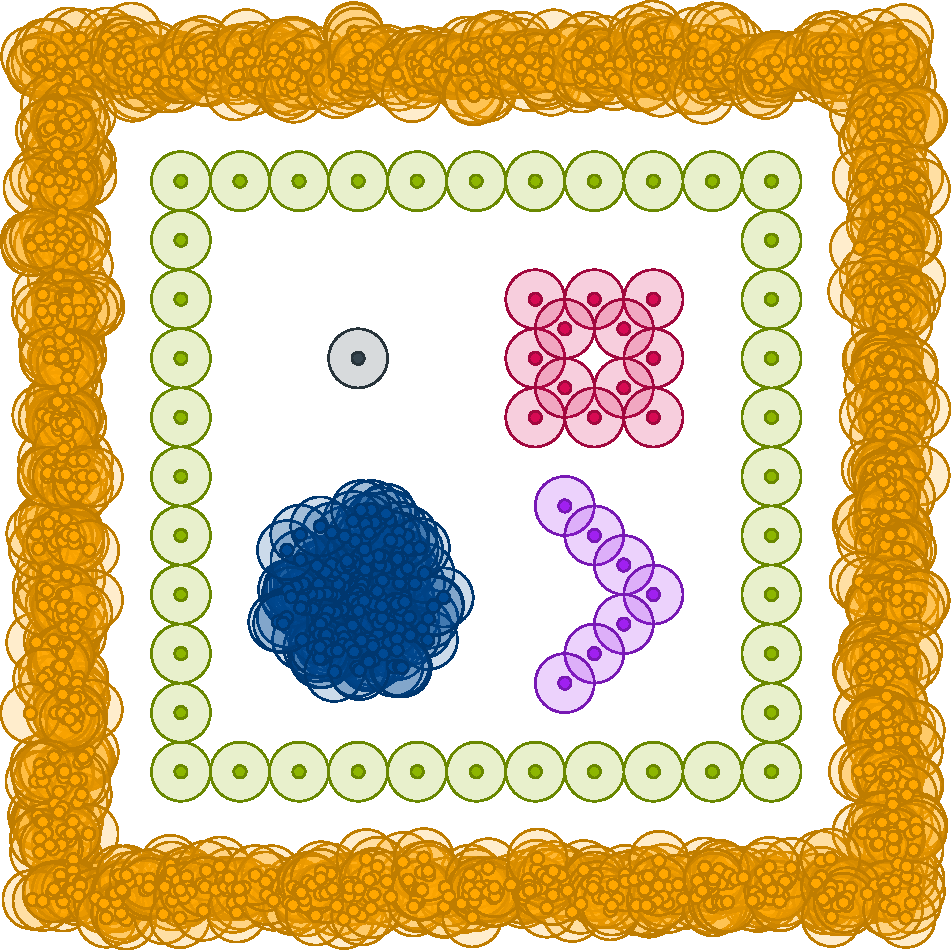
\includegraphics[width=0.8\linewidth]{Eigene/Proseminar/Cluster/en-special.pdf}\\
\midrule \phantomsection \addcontentsline{toc}{section}{Proseminar/Cluster/km-circles}\verb|Eigene/Proseminar/Cluster/km-circles|\quad{\tiny pdf}& 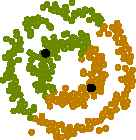
\includegraphics[width=0.8\linewidth]{Eigene/Proseminar/Cluster/km-circles.pdf}\\
\midrule \phantomsection \addcontentsline{toc}{section}{Proseminar/Cluster/km-clusters}\verb|Eigene/Proseminar/Cluster/km-clusters|\quad{\tiny pdf}& 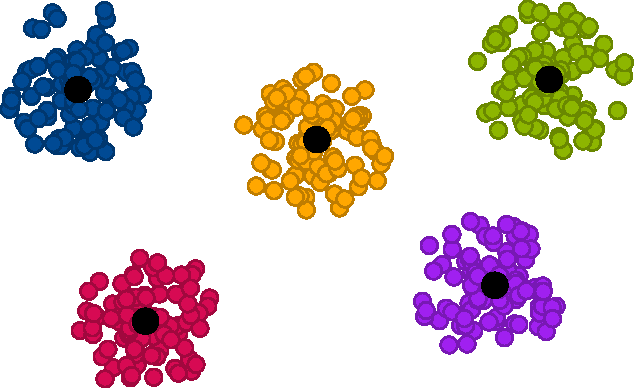
\includegraphics[width=0.8\linewidth]{Eigene/Proseminar/Cluster/km-clusters.pdf}\\
\midrule \phantomsection \addcontentsline{toc}{section}{Proseminar/Cluster/km-moons}\verb|Eigene/Proseminar/Cluster/km-moons|\quad{\tiny pdf}& 
\includegraphics[width=0.8\linewidth]{Eigene/Proseminar/Cluster/km-moons.pdf}\\
\midrule \phantomsection \addcontentsline{toc}{section}{Proseminar/Cluster/km-special}\verb|Eigene/Proseminar/Cluster/km-special|\quad{\tiny pdf}& 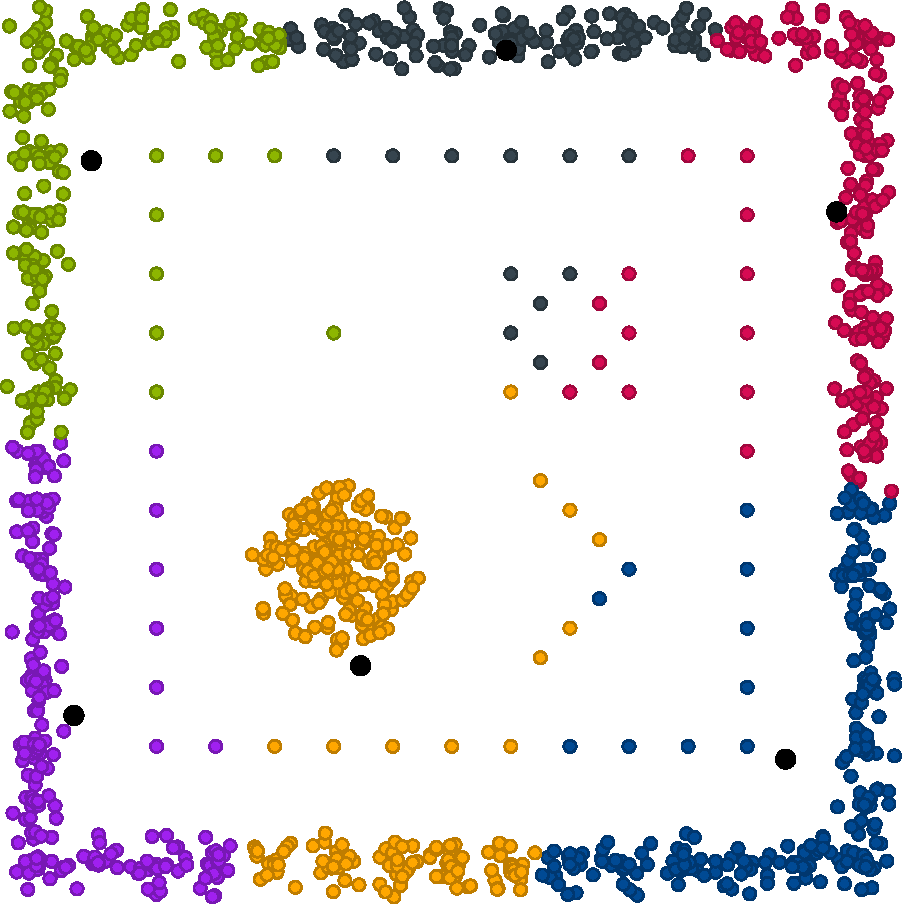
\includegraphics[width=0.8\linewidth]{Eigene/Proseminar/Cluster/km-special.pdf}\\
\midrule \phantomsection \addcontentsline{toc}{section}{Proseminar/Cluster/kn-circles}\verb|Eigene/Proseminar/Cluster/kn-circles|\quad{\tiny pdf}& 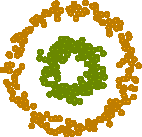
\includegraphics[width=0.8\linewidth]{Eigene/Proseminar/Cluster/kn-circles.pdf}\\
\midrule \phantomsection \addcontentsline{toc}{section}{Proseminar/Cluster/kn-clusters}\verb|Eigene/Proseminar/Cluster/kn-clusters|\quad{\tiny pdf}& 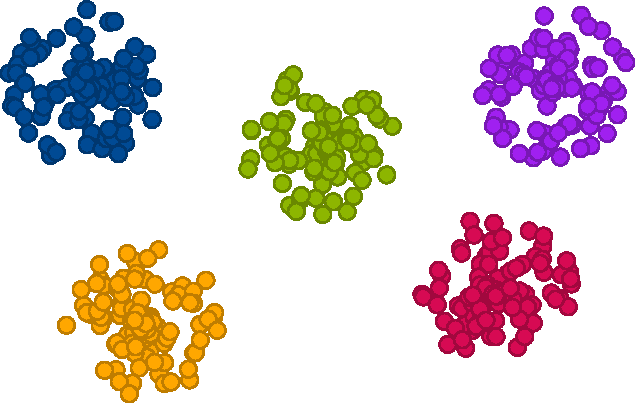
\includegraphics[width=0.8\linewidth]{Eigene/Proseminar/Cluster/kn-clusters.pdf}\\
\midrule \phantomsection \addcontentsline{toc}{section}{Proseminar/Cluster/kn-moons}\verb|Eigene/Proseminar/Cluster/kn-moons|\quad{\tiny pdf}& 
\includegraphics[width=0.8\linewidth]{Eigene/Proseminar/Cluster/kn-moons.pdf}\\
\midrule \phantomsection \addcontentsline{toc}{section}{Proseminar/Cluster/kn-special}\verb|Eigene/Proseminar/Cluster/kn-special|\quad{\tiny pdf}& 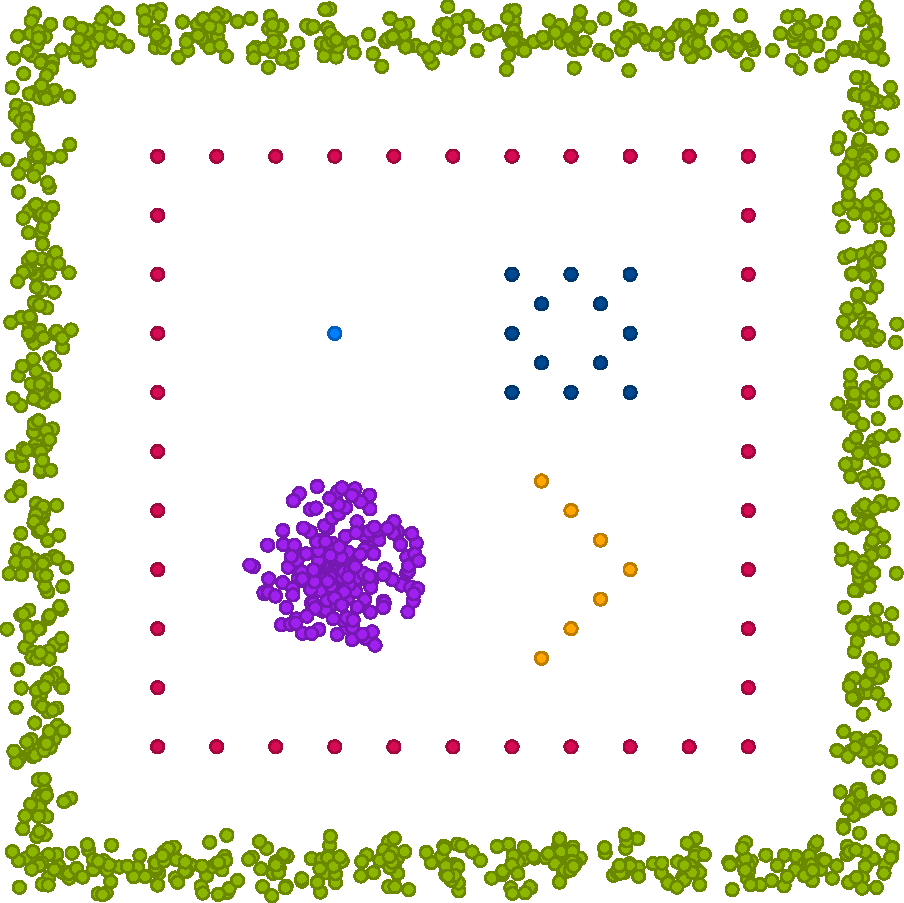
\includegraphics[width=0.8\linewidth]{Eigene/Proseminar/Cluster/kn-special.pdf}\\
\midrule \phantomsection \addcontentsline{toc}{section}{Proseminar/Cluster/rolf-circles}\verb|Eigene/Proseminar/Cluster/rolf-circles|\quad{\tiny pdf}& 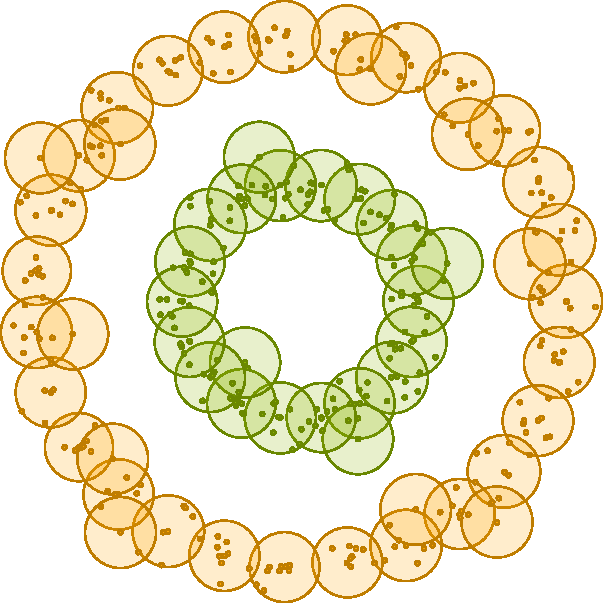
\includegraphics[width=0.8\linewidth]{Eigene/Proseminar/Cluster/rolf-circles.pdf}\\
\midrule \phantomsection \addcontentsline{toc}{section}{Proseminar/Cluster/rolf-clusters}\verb|Eigene/Proseminar/Cluster/rolf-clusters|\quad{\tiny pdf}& 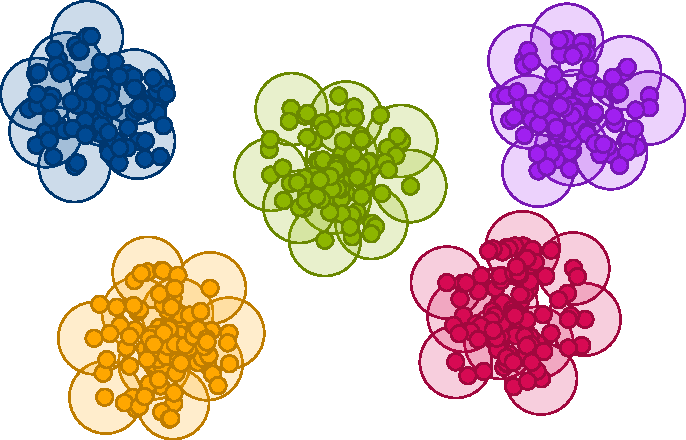
\includegraphics[width=0.8\linewidth]{Eigene/Proseminar/Cluster/rolf-clusters.pdf}\\
\midrule \phantomsection \addcontentsline{toc}{section}{Proseminar/Cluster/rolf-moons}\verb|Eigene/Proseminar/Cluster/rolf-moons|\quad{\tiny pdf}& 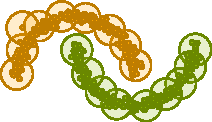
\includegraphics[width=0.8\linewidth]{Eigene/Proseminar/Cluster/rolf-moons.pdf}\\
\midrule \phantomsection \addcontentsline{toc}{section}{Proseminar/Cluster/rolf-special}\verb|Eigene/Proseminar/Cluster/rolf-special|\quad{\tiny pdf}& 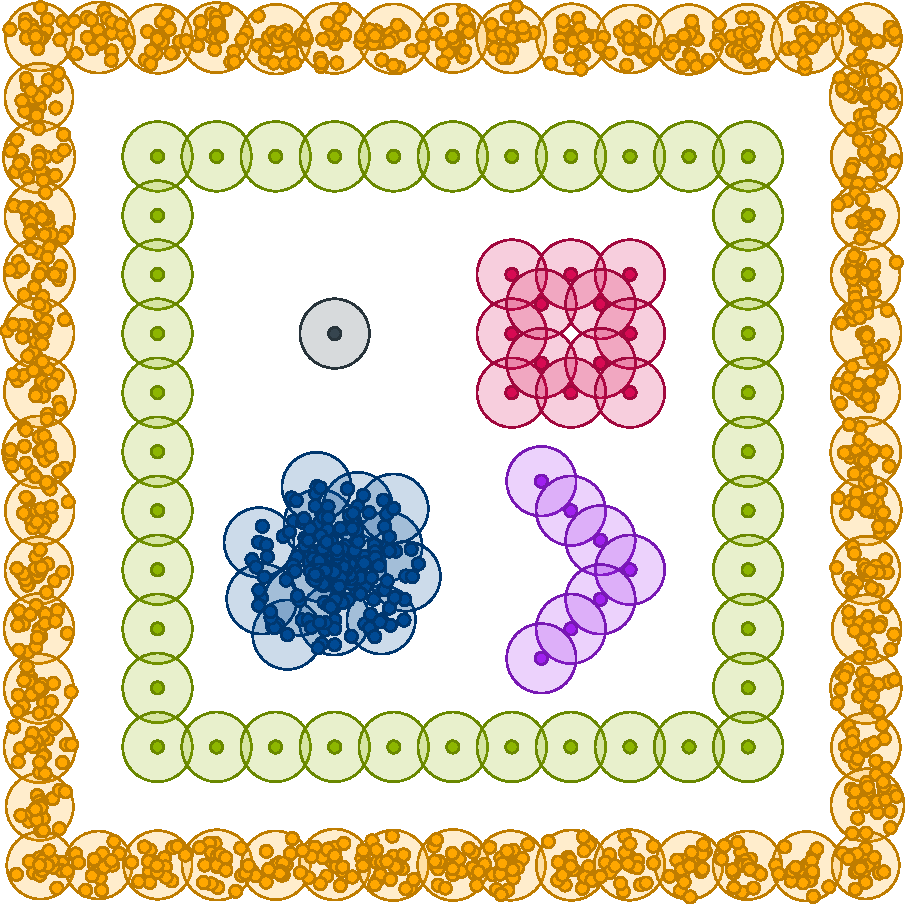
\includegraphics[width=0.8\linewidth]{Eigene/Proseminar/Cluster/rolf-special.pdf}\\
\midrule \phantomsection \addcontentsline{toc}{section}{Proseminar/Cluster/thumb-circles}\verb|Eigene/Proseminar/Cluster/thumb-circles|\quad{\tiny pdf}& 
\includegraphics[width=0.8\linewidth]{Eigene/Proseminar/Cluster/thumb-circles.pdf}\\
\midrule \phantomsection \addcontentsline{toc}{section}{Proseminar/Cluster/thumb-clusters}\verb|Eigene/Proseminar/Cluster/thumb-clusters|\quad{\tiny pdf}& 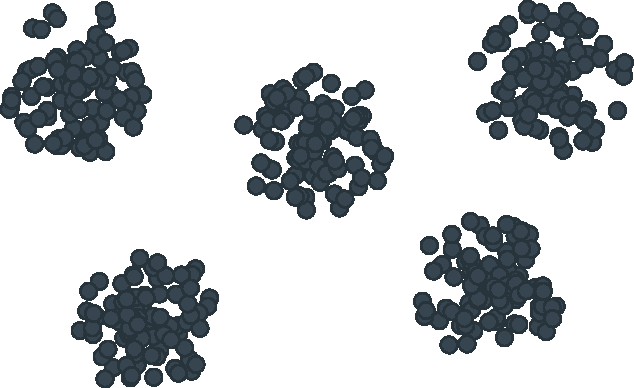
\includegraphics[width=0.8\linewidth]{Eigene/Proseminar/Cluster/thumb-clusters.pdf}\\
\midrule \phantomsection \addcontentsline{toc}{section}{Proseminar/Cluster/thumb-moons}\verb|Eigene/Proseminar/Cluster/thumb-moons|\quad{\tiny pdf}& 
\includegraphics[width=0.8\linewidth]{Eigene/Proseminar/Cluster/thumb-moons.pdf}\\
\midrule \phantomsection \addcontentsline{toc}{section}{Proseminar/Cluster/thumb-special}\verb|Eigene/Proseminar/Cluster/thumb-special|\quad{\tiny pdf}& 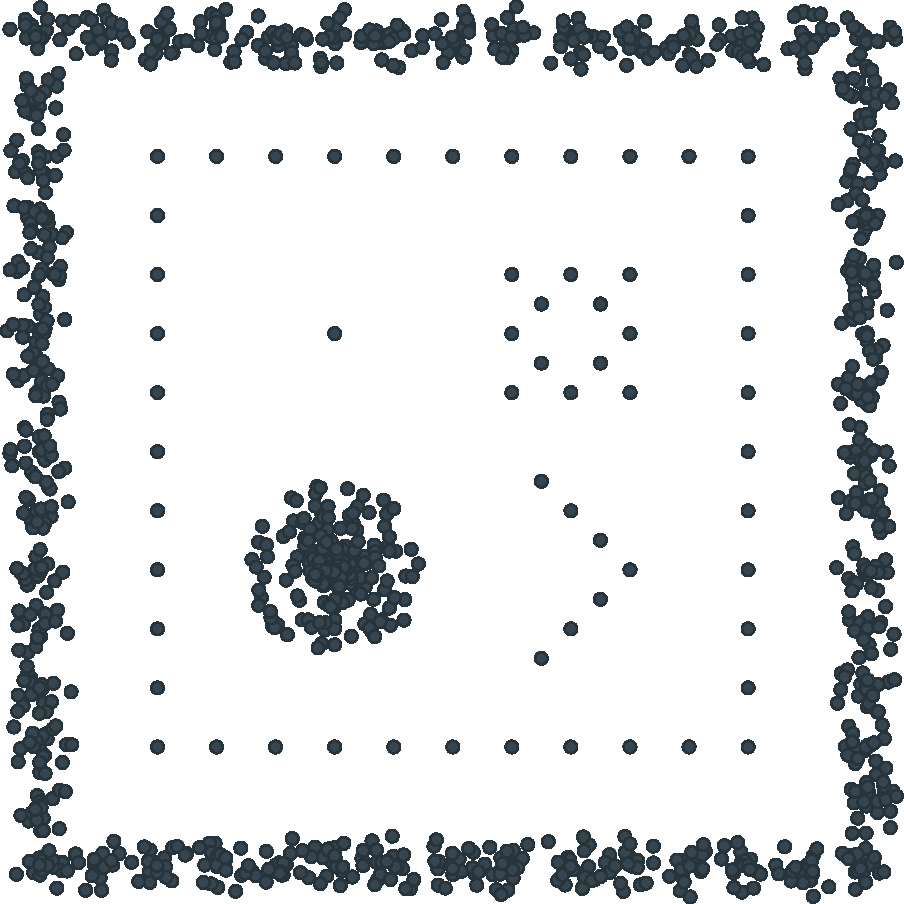
\includegraphics[width=0.8\linewidth]{Eigene/Proseminar/Cluster/thumb-special.pdf}\\
\midrule 
\phantomsection \addcontentsline{toc}{chapter}{Graphen}
\phantomsection \addcontentsline{toc}{section}{GraphNachbarschaftGrad}\verb|Graphen/GraphNachbarschaftGrad| & \getGraphics{Graphen/GraphNachbarschaftGrad}\\
\midrule \phantomsection \addcontentsline{toc}{section}{GraphNichtPlanarK33}\verb|Graphen/GraphNichtPlanarK33| & \getGraphics{Graphen/GraphNichtPlanarK33}\\
\midrule \phantomsection \addcontentsline{toc}{section}{GraphNichtPlanarK5}\verb|Graphen/GraphNichtPlanarK5| & \getGraphics{Graphen/GraphNichtPlanarK5}\\
\midrule \phantomsection \addcontentsline{toc}{section}{GraphTopologie}\verb|Graphen/GraphTopologie| & \getGraphics{Graphen/GraphTopologie}\\
\midrule \phantomsection \addcontentsline{toc}{section}{GraphWegPfad}\verb|Graphen/GraphWegPfad| & \getGraphics{Graphen/GraphWegPfad}\\
\midrule \phantomsection \addcontentsline{toc}{section}{GraphZyklus}\verb|Graphen/GraphZyklus| & \getGraphics{Graphen/GraphZyklus}\\
\midrule 
\phantomsection \addcontentsline{toc}{chapter}{Haskell}
\phantomsection \addcontentsline{toc}{section}{HaskellTypen}\verb|Haskell/HaskellTypen| & \getGraphics{Haskell/HaskellTypen}\\
\midrule \phantomsection \addcontentsline{toc}{section}{Listenoperationen}\verb|Haskell/Listenoperationen| & \getGraphics{Haskell/Listenoperationen}\\
\midrule 
\phantomsection \addcontentsline{toc}{chapter}{Java}
\phantomsection \addcontentsline{toc}{section}{StreamDemo}\verb|Java/StreamDemo| & \getGraphics{Java/StreamDemo}\\
\midrule 
\phantomsection \addcontentsline{toc}{chapter}{Logik}
\phantomsection \addcontentsline{toc}{section}{ChomskyHierarchie}\verb|Logik/ChomskyHierarchie| & \getGraphics{Logik/ChomskyHierarchie}\\
\midrule \phantomsection \addcontentsline{toc}{section}{Grammatik}\verb|Logik/Grammatik| & \getGraphics{Logik/Grammatik}\\
\midrule \phantomsection \addcontentsline{toc}{section}{KVDiagramm}\verb|Logik/KVDiagramm| & \getGraphics{Logik/KVDiagramm}\\
\midrule \phantomsection \addcontentsline{toc}{section}{KVWuerfel}\verb|Logik/KVWuerfel| & \getGraphics{Logik/KVWuerfel}\\
\midrule \phantomsection \addcontentsline{toc}{section}{QuineMCCluskeyTabelle}\verb|Logik/QuineMCCluskeyTabelle| & \getGraphics{Logik/QuineMCCluskeyTabelle}\\
\midrule \phantomsection \addcontentsline{toc}{section}{QuineMCCluskeyZusammenfassen}\verb|Logik/QuineMCCluskeyZusammenfassen| & \getGraphics{Logik/QuineMCCluskeyZusammenfassen}\\
\midrule 
\phantomsection \addcontentsline{toc}{chapter}{Prozesse}
\phantomsection \addcontentsline{toc}{section}{FCFS-WorstCase}\verb|Prozesse/FCFS-WorstCase| & \getGraphics{Prozesse/FCFS-WorstCase}\\
\midrule \phantomsection \addcontentsline{toc}{section}{FCFS}\verb|Prozesse/FCFS| & \getGraphics{Prozesse/FCFS}\\
\midrule \phantomsection \addcontentsline{toc}{section}{Prozesszustaende}\verb|Prozesse/Prozesszustaende| & \getGraphics{Prozesse/Prozesszustaende}\\
\midrule 
\phantomsection \addcontentsline{toc}{chapter}{Rechner}
\phantomsection \addcontentsline{toc}{section}{ALU}\verb|Rechner/ALU| & \getGraphics{Rechner/ALU}\\
\midrule \phantomsection \addcontentsline{toc}{section}{AmpelPLA}\verb|Rechner/AmpelPLA| & \getGraphics{Rechner/AmpelPLA}\\
\midrule \phantomsection \addcontentsline{toc}{section}{BarrelShifter}\verb|Rechner/BarrelShifter| & \getGraphics{Rechner/BarrelShifter}\\
\midrule \phantomsection \addcontentsline{toc}{section}{Beispielprozessor}\verb|Rechner/Beispielprozessor| & \getGraphics{Rechner/Beispielprozessor}\\
\midrule \phantomsection \addcontentsline{toc}{section}{CLA}\verb|Rechner/CLA| & \getGraphics{Rechner/CLA}\\
\midrule \phantomsection \addcontentsline{toc}{section}{CPLD}\verb|Rechner/CPLD| & \getGraphics{Rechner/CPLD}\\
\midrule \phantomsection \addcontentsline{toc}{section}{CSA}\verb|Rechner/CSA| & \getGraphics{Rechner/CSA}\\
\midrule \phantomsection \addcontentsline{toc}{section}{DreiTorRegister}\verb|Rechner/DreiTorRegister| & \getGraphics{Rechner/DreiTorRegister}\\
\midrule \phantomsection \addcontentsline{toc}{section}{Eintorspeicher}\verb|Rechner/Eintorspeicher| & \getGraphics{Rechner/Eintorspeicher}\\
\midrule \phantomsection \addcontentsline{toc}{section}{GALPAL}\verb|Rechner/GALPAL| & \getGraphics{Rechner/GALPAL}\\
\midrule \phantomsection \addcontentsline{toc}{section}{Geraeteverwaltung}\verb|Rechner/Geraeteverwaltung| & \getGraphics{Rechner/Geraeteverwaltung}\\
\midrule \phantomsection \addcontentsline{toc}{section}{HardwareSkizze}\verb|Rechner/HardwareSkizze| & \getGraphics{Rechner/HardwareSkizze}\\
\midrule \phantomsection \addcontentsline{toc}{section}{ISA}\verb|Rechner/ISA| & \getGraphics{Rechner/ISA}\\
\midrule \phantomsection \addcontentsline{toc}{section}{LUT}\verb|Rechner/LUT| & \getGraphics{Rechner/LUT}\\
\midrule \phantomsection \addcontentsline{toc}{section}{LUTOder}\verb|Rechner/LUTOder| & \getGraphics{Rechner/LUTOder}\\
\midrule \phantomsection \addcontentsline{toc}{section}{MIPS}\verb|Rechner/MIPS| & \getGraphics{Rechner/MIPS}\\
\midrule \phantomsection \addcontentsline{toc}{section}{MuxDemuxKommunikation}\verb|Rechner/MuxDemuxKommunikation| & \getGraphics{Rechner/MuxDemuxKommunikation}\\
\midrule \phantomsection \addcontentsline{toc}{section}{MuxShannon}\verb|Rechner/MuxShannon| & \getGraphics{Rechner/MuxShannon}\\
\midrule \phantomsection \addcontentsline{toc}{section}{NAdressmaschiene}\verb|Rechner/NAdressmaschiene| & \getGraphics{Rechner/NAdressmaschiene}\\
\midrule \phantomsection \addcontentsline{toc}{section}{PLA}\verb|Rechner/PLA| & \getGraphics{Rechner/PLA}\\
\midrule \phantomsection \addcontentsline{toc}{section}{PLAZuAmpel}\verb|Rechner/PLAZuAmpel| & \getGraphics{Rechner/PLAZuAmpel}\\
\midrule \phantomsection \addcontentsline{toc}{section}{PROM}\verb|Rechner/PROM| & \getGraphics{Rechner/PROM}\\
\midrule \phantomsection \addcontentsline{toc}{section}{Pages}\verb|Rechner/Pages| & \getGraphics{Rechner/Pages}\\
\midrule \phantomsection \addcontentsline{toc}{section}{Physik/DiodenStromstaerke}\verb|Rechner/Physik/DiodenStromstaerke| & \getGraphics{Rechner/Physik/DiodenStromstaerke}\\
\midrule \phantomsection \addcontentsline{toc}{section}{Physik/Metastabil}\verb|Rechner/Physik/Metastabil| & \getGraphics{Rechner/Physik/Metastabil}\\
\midrule \phantomsection \addcontentsline{toc}{section}{Physik/TransistorStoertoleranz}\verb|Rechner/Physik/TransistorStoertoleranz| & \getGraphics{Rechner/Physik/TransistorStoertoleranz}\\
\midrule \phantomsection \addcontentsline{toc}{section}{RegisterParallel}\verb|Rechner/RegisterParallel| & \getGraphics{Rechner/RegisterParallel}\\
\midrule \phantomsection \addcontentsline{toc}{section}{RegisterSeriell}\verb|Rechner/RegisterSeriell| & \getGraphics{Rechner/RegisterSeriell}\\
\midrule \phantomsection \addcontentsline{toc}{section}{Shiftregister}\verb|Rechner/Shiftregister| & \getGraphics{Rechner/Shiftregister}\\
\midrule \phantomsection \addcontentsline{toc}{section}{Speicherhierarchie}\verb|Rechner/Speicherhierarchie| & \getGraphics{Rechner/Speicherhierarchie}\\
\midrule \phantomsection \addcontentsline{toc}{section}{StackExample}\verb|Rechner/StackExample| & \getGraphics{Rechner/StackExample}\\
\midrule \phantomsection \addcontentsline{toc}{section}{Stackmaschiene}\verb|Rechner/Stackmaschiene| & \getGraphics{Rechner/Stackmaschiene}\\
\midrule \phantomsection \addcontentsline{toc}{section}{StackmaschieneSimpler}\verb|Rechner/StackmaschieneSimpler| & \getGraphics{Rechner/StackmaschieneSimpler}\\
\midrule 
\phantomsection \addcontentsline{toc}{chapter}{Schaltkreis}
\phantomsection \addcontentsline{toc}{section}{Addier-Subtrahierer}\verb|Schaltkreis/Addier-Subtrahierer| & \getGraphics{Schaltkreis/Addier-Subtrahierer}\\
\midrule \phantomsection \addcontentsline{toc}{section}{Demultiplexer}\verb|Schaltkreis/Demultiplexer| & \getGraphics{Schaltkreis/Demultiplexer}\\
\midrule \phantomsection \addcontentsline{toc}{section}{SynchronzaehlerDFF}\verb|Schaltkreis/SynchronzaehlerDFF| & \getGraphics{Schaltkreis/SynchronzaehlerDFF}\\
\midrule \phantomsection \addcontentsline{toc}{section}{SynchronzaehlerTFF}\verb|Schaltkreis/SynchronzaehlerTFF| & \getGraphics{Schaltkreis/SynchronzaehlerTFF}\\
\midrule \phantomsection \addcontentsline{toc}{section}{Volladdierer}\verb|Schaltkreis/Volladdierer| & \getGraphics{Schaltkreis/Volladdierer}\\
\midrule 
\phantomsection \addcontentsline{toc}{chapter}{Software}
\phantomsection \addcontentsline{toc}{section}{DreiSchichtenArchitektur}\verb|Software/DreiSchichtenArchitektur| & \getGraphics{Software/DreiSchichtenArchitektur}\\
\midrule \phantomsection \addcontentsline{toc}{section}{Meta/ProgrammierparadigmenUeberblick}\verb|Software/Meta/ProgrammierparadigmenUeberblick| & \getGraphics{Software/Meta/ProgrammierparadigmenUeberblick}\\
\midrule \phantomsection \addcontentsline{toc}{section}{ModelViewController}\verb|Software/ModelViewController| & \getGraphics{Software/ModelViewController}\\
\midrule \phantomsection \addcontentsline{toc}{section}{RegexExample}\verb|Software/RegexExample| & \getGraphics{Software/RegexExample}\\
\midrule \phantomsection \addcontentsline{toc}{section}{ThreadStates}\verb|Software/ThreadStates| & \getGraphics{Software/ThreadStates}\\
\midrule \phantomsection \addcontentsline{toc}{section}{UMLCompositePattern}\verb|Software/UMLCompositePattern| & \getGraphics{Software/UMLCompositePattern}\\
\midrule \phantomsection \addcontentsline{toc}{section}{UMLDecoratorPattern}\verb|Software/UMLDecoratorPattern| & \getGraphics{Software/UMLDecoratorPattern}\\
\midrule \phantomsection \addcontentsline{toc}{section}{UMLExample}\verb|Software/UMLExample| & \getGraphics{Software/UMLExample}\\
\midrule \phantomsection \addcontentsline{toc}{section}{UMLObserverPattern}\verb|Software/UMLObserverPattern| & \getGraphics{Software/UMLObserverPattern}\\
\midrule \phantomsection \addcontentsline{toc}{section}{UMLSEQObserverPattern}\verb|Software/UMLSEQObserverPattern| & \getGraphics{Software/UMLSEQObserverPattern}\\
\midrule \phantomsection \addcontentsline{toc}{section}{UMLSEQObserverPatternAdapted}\verb|Software/UMLSEQObserverPatternAdapted| & \getGraphics{Software/UMLSEQObserverPatternAdapted}\\
\midrule \phantomsection \addcontentsline{toc}{section}{UMLStateDiagramExample}\verb|Software/UMLStateDiagramExample| & \getGraphics{Software/UMLStateDiagramExample}\\
\midrule \phantomsection \addcontentsline{toc}{section}{UMLThread}\verb|Software/UMLThread| & \getGraphics{Software/UMLThread}\\
\midrule \bottomrule
\end{tabularx}
\end{document}